\documentclass{beamer}
\usetheme{Boadilla}

\title{Pythagorean theorem}
\author{M.Amin Roshani}
\institute{University of Tehran}
\date{\today}

\begin{document}


\maketitle




\begin{frame}
\tableofcontents
\end{frame}

\begin{frame}
\frametitle{Abstract}
\section{Abstract}
In mathematics, the Pythagorean theorem, also known as Pythagoras' theorem, is a fundamental relation in Euclidean geometry among the three sides of a right triangle. It states that the area of the square whose side is the hypotenuse (the side opposite the right angle) is equal to the sum of the areas of the squares on the other two sides. This theorem can be written as an equation relating the lengths of the sides a, b and c, often called the "Pythagorean equation".
\end{frame}

\begin{frame}
\frametitle{Rearrangement proof}
\section{Rearrangement proof}
\label{sec1}
\begin{figure}[H]
    \centering
    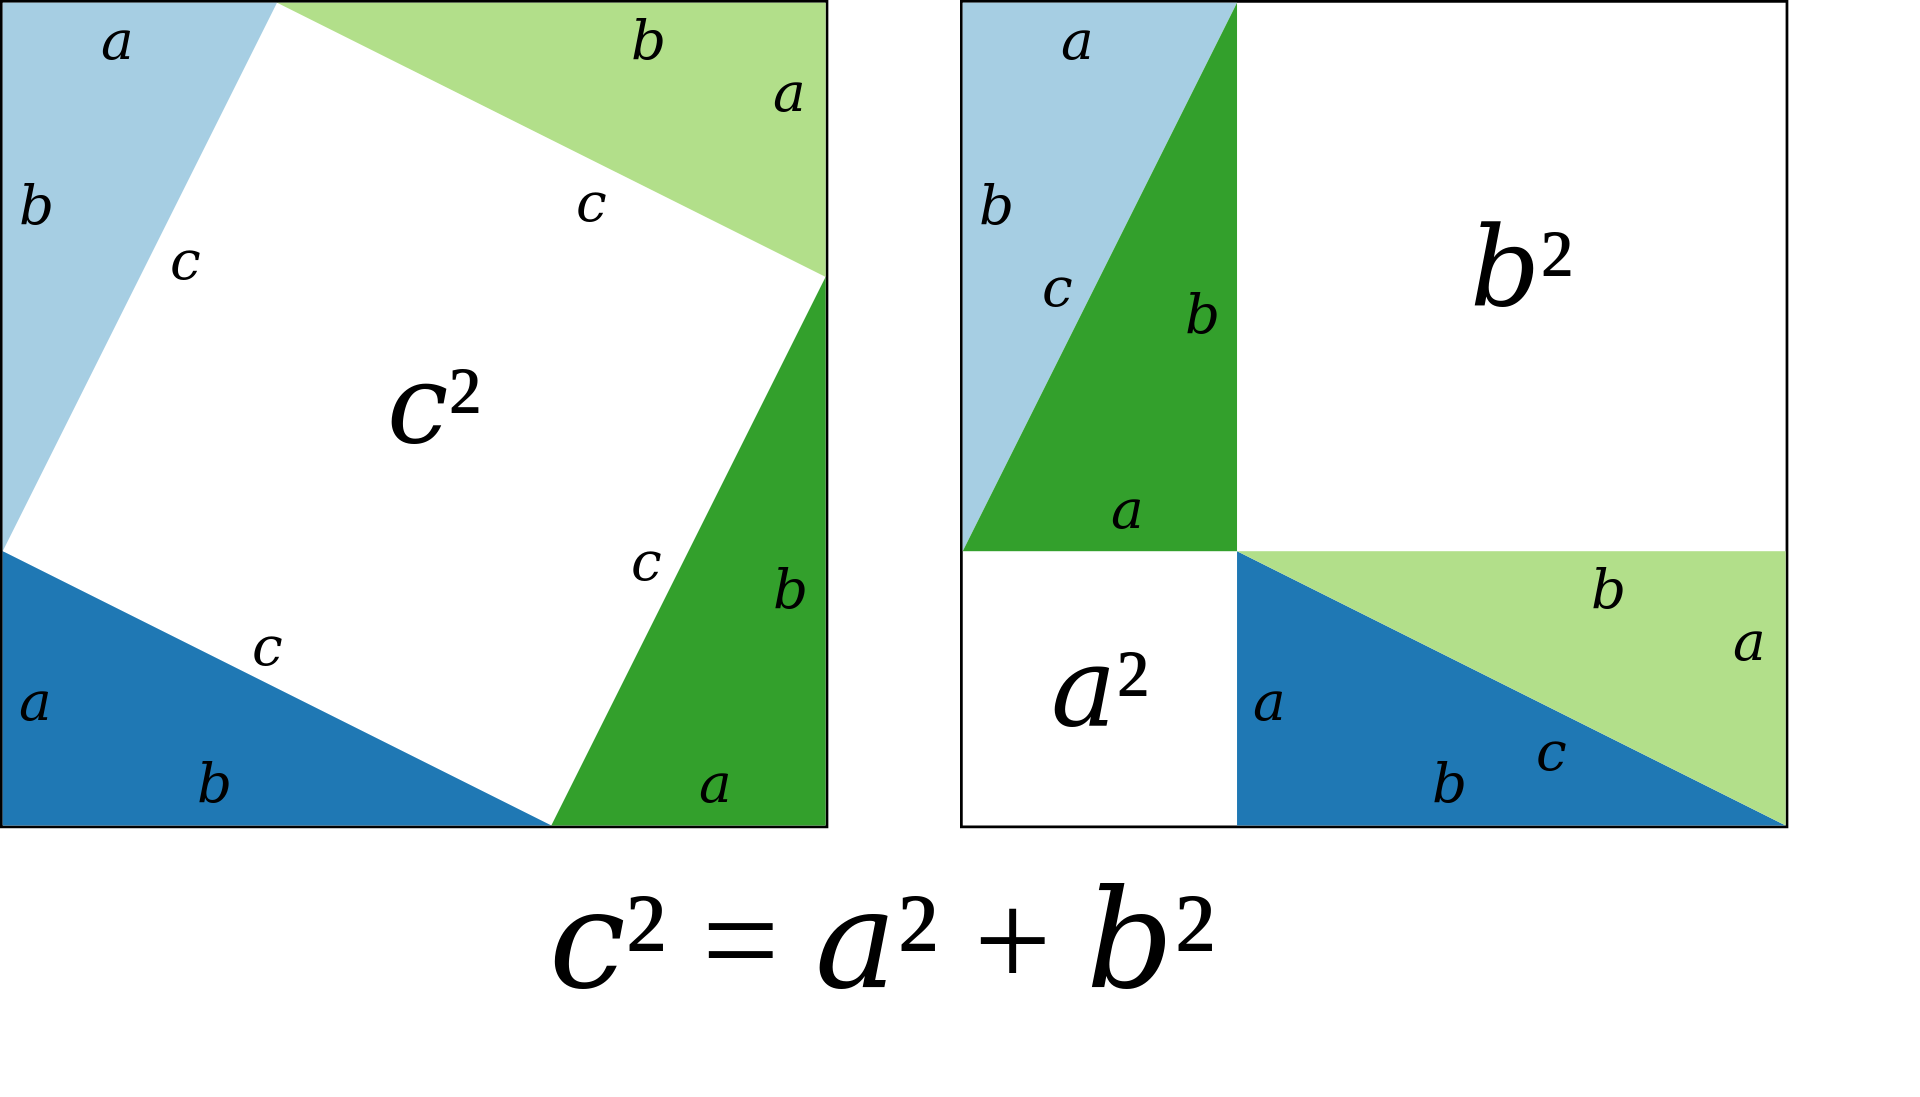
\includegraphics[scale=0.12]{figs/Pythagoras-proof-anim.svg.png} \\
    \caption{The rearrangement proof}
    \label{fig:my_label}
\end{figure}
\begin{equation}
    c = \sqrt{a^2 + b^2}
\end{equation}
\begin{equation}
    \sqrt{(a_1 + a_1)^2 + (a_2 + a_2)^2 + (a_n + a_n)^2} = \sqrt{\sum_{i=1}^{n} (a_i - b_i)^2}
\end{equation}
\end{frame}
\begin{frame}
\frametitle{Extra explanation}
\subsection{Extra explanation}
The Pythagorean equation relates the sides of a right triangle in a simple way, so that if the lengths of any two sides are known the length of the third side can be found. Another corollary of the theorem is that in any right triangle, the hypotenuse is greater than any one of the other sides, but less than their sum.
\end{frame}

\begin{frame}
\frametitle{List of some proofs}
\section{List of some proofs}
\begin{enumerate}
     \item Proof using similar triangles
    \item Euclid's proof
    \item Proofs by dissection and rearrangement
    \item Einstein's proof by dissection without rearrangement
    \item Algebraic proofs
\end{enumerate}
\end{frame}

\begin{frame}
\frametitle{Table of proofs}
\subsection{Table of proofs}
\begin{center}
 \begin{tabular}{||c | c||} 
\hline
 1 & Proof using similar triangles \\ 
 \hline
 2 & Euclid's proof \\
 \hline
 3 & Proofs by dissection and rearrangement \\
 \hline
 4 & Einstein's proof by dissection without rearrangement \\
 \hline
 5 & Algebraic proofs \\ [1ex] 
 \hline
\end{tabular}
\newline
\end{center}
\end{frame}


\end{document}
